%!TEX root = ../../thesis.tex
\chapter{Bacteriophage Mosaicism}
\label{ch:phage}

\section{Introduction}
\label{phage:sec:introduction}

Bacteriophages, bacteria-infecting viruses, are the most abundant organism on the planet: $10^31$ organisms [cite].
\kje{[More background info: metagenomics, ocean phage, etc.]}
The current bacteriophage taxonomy is compiled by the International Committee on Taxonomy of Viruses (ICTV) and is based on virus morphology, host range, lifestyle, and nucleic acid composition \cite{ICTV:2012}.
Unlike the constituents of the generall accepted tree of life, phages lack a universal replicative machinery, rRNA, that can be used to define a species tree.
Nucleic acid composition is either double-stranded DNA (dsDNA), single-stranded DNA (ssDNA), double-stranded RNA (dsRNA), or single-stranded RNA (ssRNA).
Of these dsDNA is by far the most common.
Morphological classification is primarily based on head/capsid shape and tail length.
Table~\ref{phage:table:families} presents an overview of phage families defined by the ICTV.

\begin{table}[t]
    \caption{Phage families defined by the ICTV}
    \centering
    \scriptsize
    \begin{tabularx}{\textwidth}{lXlX}
    \toprule
    Order & Family & Morphology & Nucleic acid \\
    \midrule
    \multirow{3}{*}{\emph{Caudovirales}} & \emph{Myoviridae} & Nonenveloped, contractile tail & linear dsDNA \\
                                  & \emph{Siphoviridae} & Nonenveloped, noncontractile tail (long) & linear dsDNA \\
                                  & \emph{Podoviridae} & Nonenveloped, noncontractile tail (short) & linear dsDNA \\
    \midrule
    \multirow{2}{*}{\emph{Ligamenvirales}} & \emph{Lipothrixviridae} & Enveloped, rod-shaped & linear dsDNA \\
                                    & \emph{Rudiviridae} & Nonenveloped, rod-shaped & linear dsDNA \\
    \midrule
    \multirow{13}{*}{Unassigned} & \emph{Ampullaviridae} & Enveloped, bottle-shaped & linear dsDNA\\
                                 & \emph{Bicaudaviridae} & Nonenveloped, lemon-shaped & circular dsDNA \\
                                 & \emph{Clavaviridae}   & Nonenveloped, rod-shaped & circular dsDNA \\
                                 & \emph{Corticoviridae} & Nonenveloped, isometric & circular dsDNA \\
                                 & \emph{Cystoviridae}   & Enveloped, spherical & segmented dsRNA \\
                                 & \emph{Fuselloviridae} & Nonenveloped, lemon-shaped & circular dsDNA \\
                                 & \emph{Globuloviridae} & Enveloped, isometric& linear dsDNA \\
                                 & \emph{Guttaviridae}   & Nonenveloped, ovoid & circular dsDNA \\
                                 & \emph{Inoviridae}     & Nonenveloped, filamentou& circular ssDNA \\
                                 & \emph{Leviviridae}    & Nonenveloped, isometric & linear ssRNA \\
                                 & \emph{Microviridae}   & Nonenveloped, isometric & circular ssDNA \\
                                 & \emph{Plasmaviridae}  & Enveloped, pleomorph& circular dsDNA \\
                                 & \emph{Tectiviridae}   & Nonenveloped, isometric & linear dsDNA \\
    \bottomrule
    \end{tabularx}
    \label{phage:table:families}
\end{table}

It has long been known that phage species are genetic mosaics with extremeley high rates of lateral exchange.
The advent of genome sequencing solidified this observation and brought to bear questions about the applicability and interpretation of the ICTV taxonomy.
Unlike prokaryotes and eukaryotes, phages do not have ribosomal RNA.
Indeed there is substantial debate over whether phages are truly alive and whether or not they should be a component in the tree of life.
Given the substantial amount of genetic diversity 

The current bacteriophage taxonomy is inconsistent with recently collected genomic data.
In Figure~\ref{phage:fig:inconsistency} we see three different bacteriophage species.
HK97 is a Siphoviridae infecting \emph{E. coli}.
L5 is a Siphoviridae infecting \emph{M. smegmatis}.
P22 is a Podoviridae infecting \emph{S. enterica}.
HK97 and L5 belong to the Siphoviridae family comprised of long tail noncontracile phages.
P22 belongs to the Podoviridae family comprised of short tail phages.
Visually, it appears that HK97 and L5 should indeed be classified as distinct from P22.
However, genomic analysis indicates that HK97 and L5 share no gene content.
Despite belonging to different viral families, HK97 and P22 share 20\% gene content.
If we are to take genomic data as the core information defining.

\begin{figure}
\centering
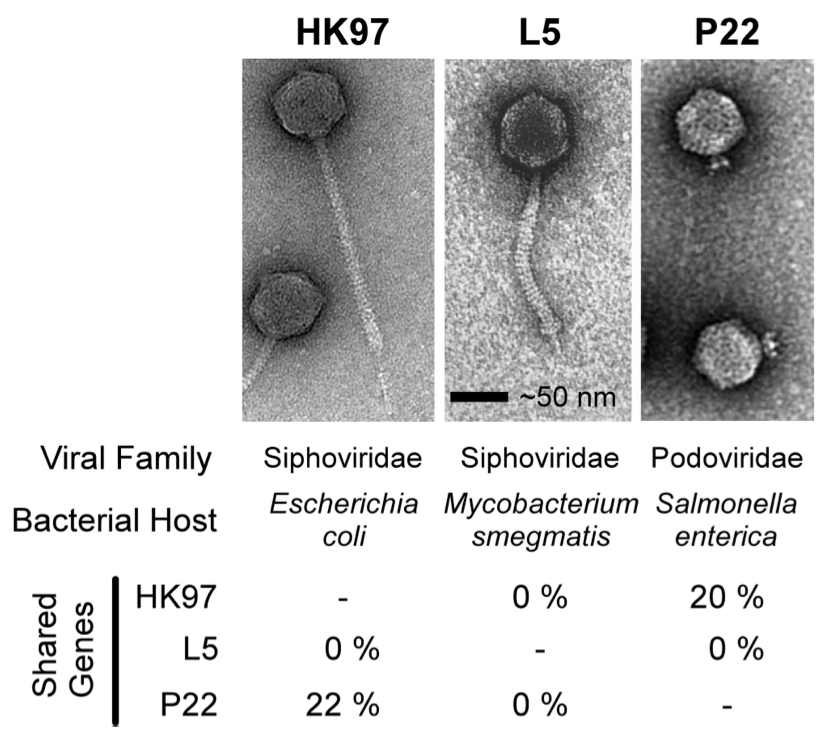
\includegraphics[width=.5\linewidth]{./fig/LAWRENCE_phage_comparative.png}
\caption[Inconsistency of morphological classification in bacteriophage.]{Inconsistency of genomic and morphological approaches. HK97 and L5 are classified under same viral family, despite sharing no homologous genetic content. P22 on the other hand shares many genes. Figure adapted from \parencite{Lawrence:2002eg}}
\label{phage:fig:inconsistency}
\end{figure}

Alternatives have been proposed based on whole genome analysis.
For example, see Rohwer and Edwards and the phage proteomic tree \cite{Rohwer:2002uo}.
However, these models still broadly assume a tree like structure.

In this chapter, we use topological approaches to define a systematic way of structuring phage relationships based on gene content.
This work is based on data collected by Lima-Mendea \emph{et al.} \cite{LimaMendez:2008ki} and Kristensen \emph{et al.} \cite{Kristensen:2013tt}.
First, we use persistent homology to characterize reticulation in phage genomes.
We find $H_0$ consistent with existing phage taxonomies.
We interpret $H_1$ as evidence for genetic exchange due to shared ecology and host-range. 
Second, we visualize phage relationships using mapper, identifying non-obvious relationships between phages of varying nucleic acid content.

\section{Approach}
\label{phage:sec:approach}

\subsection{Data}

First data set follows that from \cite{LimaMendez:2008ki}
Input data is 306 bacteriophage genomes.
250 dsDNA, 36 ssDNA, 12 dsRNA, and 8 ssRNA.
1,9537 genes clustered into 8,576 gene families using BlastP.
Construct Phyletic profile: nxp binary gene presence/absence matrix.
29 outlier phages, discard and keep only subset S277.

Second data set follows that from \cite{Kristensen:2013tt} and is more extensive.
This dataset defines phage orthologous groups (POGs) and includes viruses of prokaryotic host including bacteria and archaea.
Input data is 1,005 phage genomes.

\section{Results}
\label{phage:sec:results}

We show the barcode diagrams in Figure~\ref{phage:fig:limamendez_barcode}.
$H_0$ gives an initial classification.
Cycles in $H_1$ can be mapped to specific reticulation patterns.
These cycles reflect shared environment.

\begin{figure}
\centering
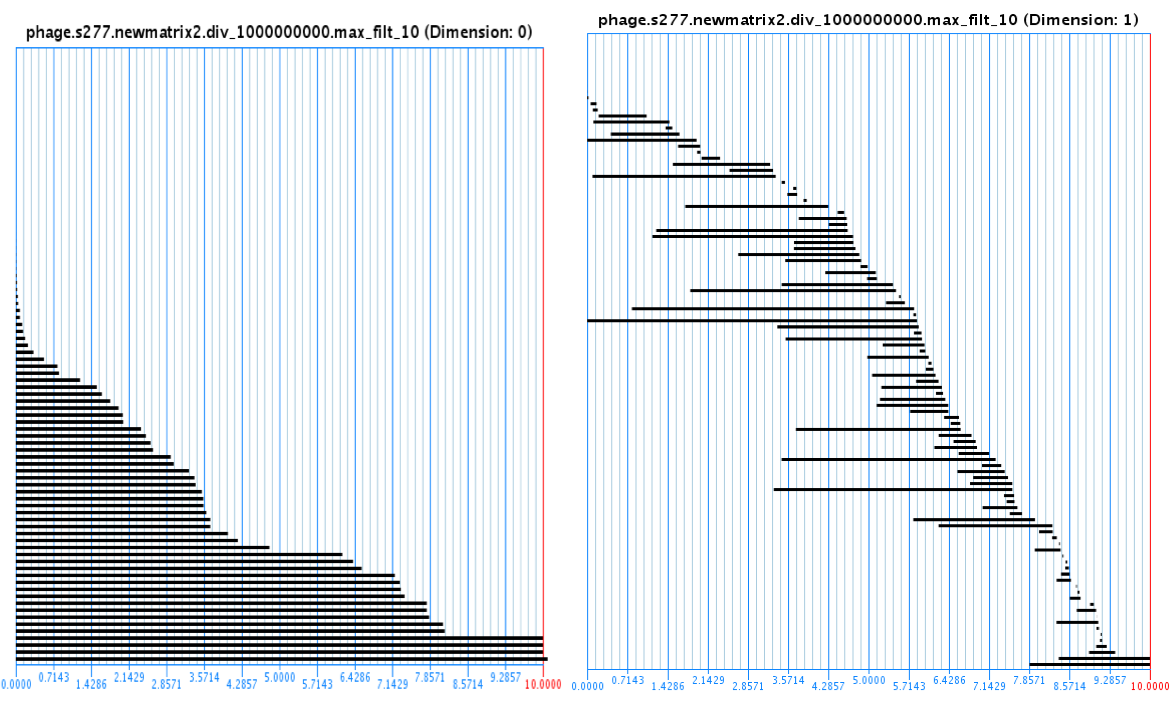
\includegraphics[width=.8\linewidth]{./fig/limamendez_barcode.png}
\caption[Bacteriophage Barcode Diagram]{Bacteriophage Barcode Diagram using the Lima-Mendez dataset.}
\label{phage:fig:limamendez_barcode}
\end{figure}

In Figure~XXX we show the barcode diagram.
We show the relationship of these bars within an existing phage taxonomy.
Extract multiscale patterns of reticulation.
Phage phylogeny taken from \cite{Glazko:2007dc}.

Finally, we use Ayasdi Iris to construct a network visualization of the phage phyletic profiles.
We see several interesting things.
Using Ayasdi, we can identify gene enrichment in particular clusters.
We can also correlate with lifestyle and ecological properties.

\section{Phage Ecological Properties}
\label{phage:sec:ecological_properties}

We can associate particular generators with ecological groupings.

\section{Conclusions}
\label{phage:sec:conclusions}

We showed that we can charact